\subsubsection{MULTI-SCALE 3D INTERPRETATION}
To understand this technique we need to analyse the same target in 
two different positions, as in Fig. \ref{fig:multiscale3d}.

\begin{figure}[H]
\centering
  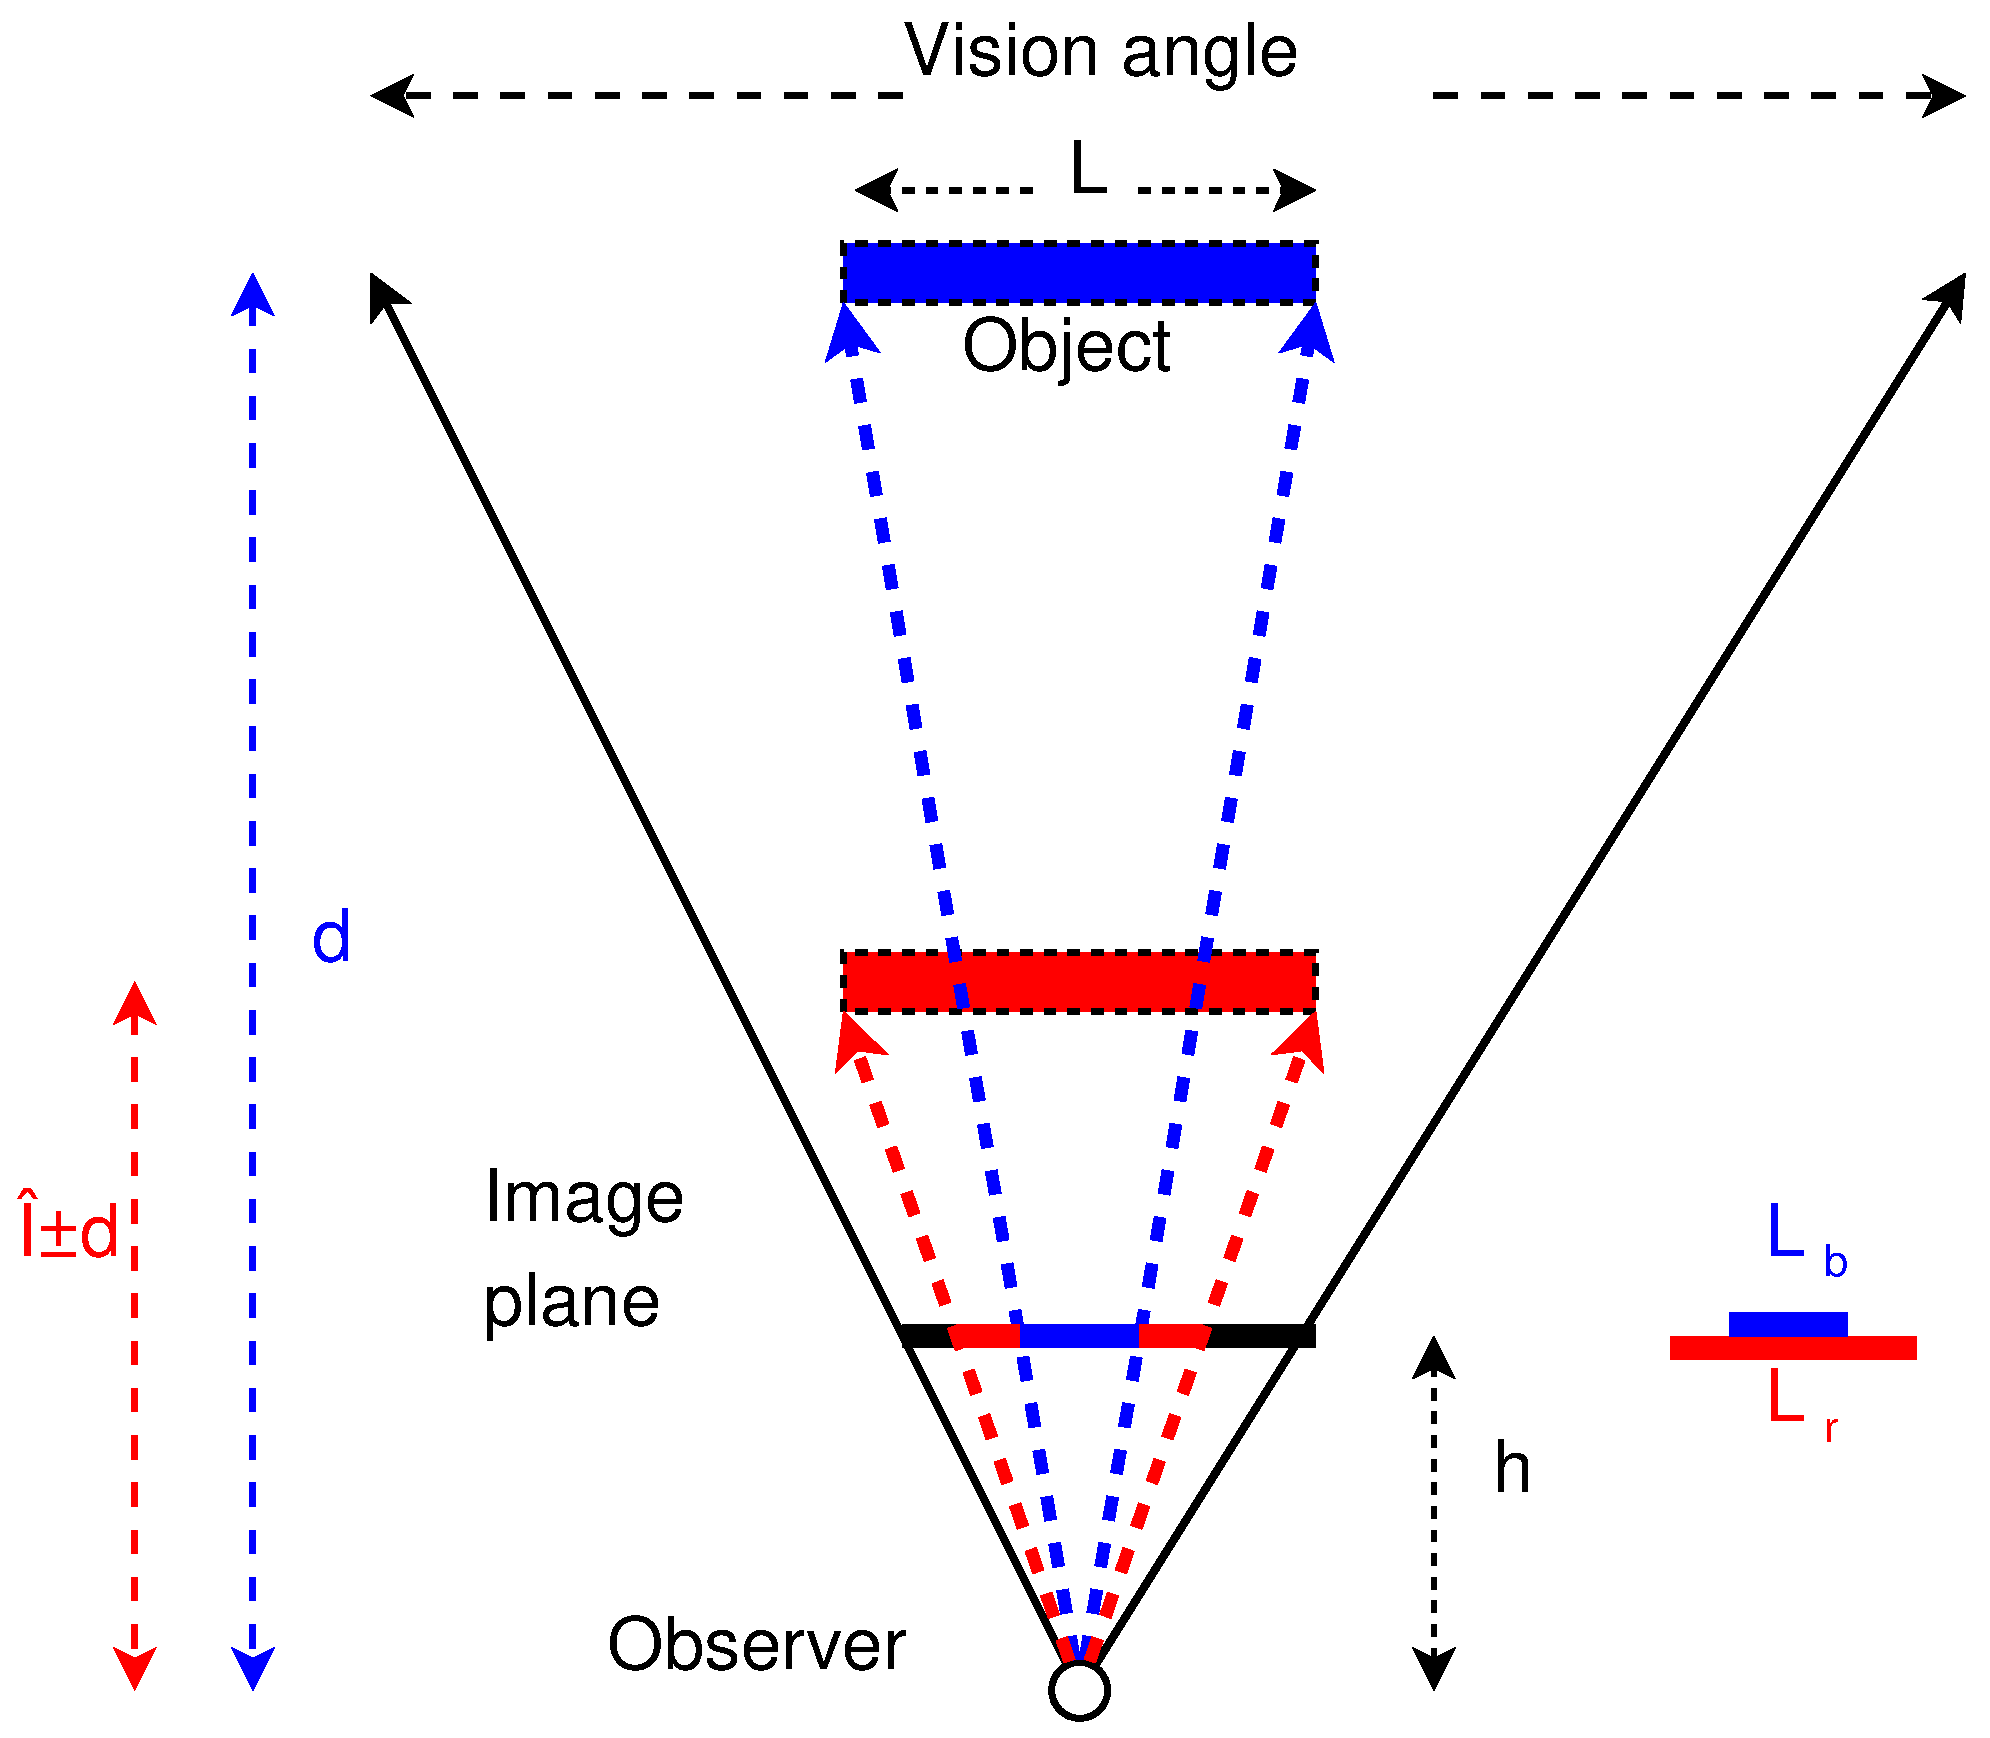
\includegraphics[width=.7\columnwidth]{images/Diagrama3.eps}
  \caption{The multi-scale tracking.}
  \label{fig:multiscale3d}
\end{figure}

Fig.\ref{fig:multiscale3d} shows the same target at two different distances $d$ and $\alpha d$, respectively, in blue and red.
The image plane is located at a distance $h$ of the observer.
The projections of objects, in blue and red, are labelled in the image as
$L_b$ and $L_r$, respectively. Making a simple inspection in the
formed triangles, we can see that $\frac{h}{d}=\frac{L_b}{L}$ and 
$\frac{h}{\alpha d}=\frac{L_r}{L}$, then $L_b/\alpha= L_r$. 
From the point of view of the observer, this implies that when a target 
is located at a distance $d$ at a time $t_0$,  and a distance $\alpha d$ at a time $t_1$, 
the width of the target in the image plane is altered by a factor of 1/$\alpha$, 
and consequently its area is altered by a factor of 1/$\alpha^2$.

The criterion method the searches for objects using different discrete values of $\alpha$. 
The algorithm tracks the nearest objects with $\alpha<1$ and objects farthest with $\alpha>1$.

%usa Multi-resolution match criteria e explica isso dos tamanhos

\subsubsection{DEPARTURE FACTOR - RELATIVE VELOCITY}
The departure factor is a dimensionless number related to the rate of approach 
or departure of a target to the observer. The factor
is determined in \ref{eq:relarea},

\begin{equation}\label{eq:relarea}
f_a \equiv \alpha^2 \equiv \frac{Area_r}{Area_f} 
\end{equation}

where $f_a$ and $\alpha$ are defined as factor area and departure factor, 
respectively; $Area_r$ is the ROI area and $Area_f$ 
is the analyzed region in the current image frame.

Thus, knowing $\alpha$, if we consider that the target in the $ROI$ was to a distance $d_0$,
then the target in the analysis region will be to a distance of $\alpha d_0$ (or $\sqrt{f_a} d_0$).
So that, each $i-th$ frame will have its own $\alpha_i$ value; where, $d_i=\alpha_i d_0$.

The departure factor, $\alpha_i$, has two interpretations: if the rate of departure increases quickly, 
this  means that the target is departing. If the factor decreases, the 
target is approaching.

The relative velocity is using a simple equation of kinematic in physics:
\begin{equation}
 v_i = \frac{\Delta s}{\Delta t}= \frac{s_i-s_{i-1}}{\Delta t}.
\end{equation}

where the vector $v_i$ represents the relative velocity in the i-th image frame, 
$s_i=(x_i,y_i,d_i)$ is the position of match in the i-th image frame
and $\Delta t$ is the sampling time between image frames.
Additionally, we call velocity of departure factor, $v^d_i$, 
the scalar number which represents the depth component
of the vector $v_i$.

The calculated  $v^d_i$ value is relative, for the simple reason that the distance (depth) between the 
camera (observer) and the target in the instance i-th will be referenced to $d_0$, 
given that the distance of the initial $ROI$ is established by definition to 1.
Finally, in all cases, the position $s_i$ is relative to the observer (a moving reference system).

